\chapter{Конструкторская часть}

Ранее в этой секции были представлены рекуррентные формулы, которые позволяют вычислять расстояние Левенштейна и Дамерау - Левенштейна. 
Однако, при разработке алгоритмов для решения этих задач, доступны различные подходы, такие как итеративный алгоритм, алгоритм рекурсии с использованием кэширования и алгоритм рекурсии без кэширования. 
В данной части рассмотрим каждый из этих подходов более подробно. 
Также в данной части указываются требования к программному обеспечению (ПО).

\section{Требования к программному обеспечению}

Программе передаются две строки в качестве входных данных, и она должна вычислить и вывести искомое расстояние, используя каждый из реализованных алгоритмов: для Левенштейна -- итеративный, для Дамерау - Левенштейна -- итеративный, рекурсивный без использования кэша и рекурсивный с использованием кэша. 
Кроме того, необходимо сообщить затраченное каждым алгоритмом процессорное время и память.

В создаваемом приложении пользователю должны быть доступны функции ввода двух строк и выбора желаемого алгоритма. Пользователь должен иметь возможность оценить размер и работу каждого алгоритма.

\section{Алгоритм поиска расстояния Левенштейна}

Для оптимизации нахождения расстояния Левенштейна можно использовать матрицу в целях хранения соответствующих промежуточных значений. 
В таком случае алгоритм представляет собой построчное заполнение матрицы. 

На рисунке~\ref{fig:Levenstain} приведена схема рассматриваемого алгоритма.

\begin{figure}[h]
	
	\centering{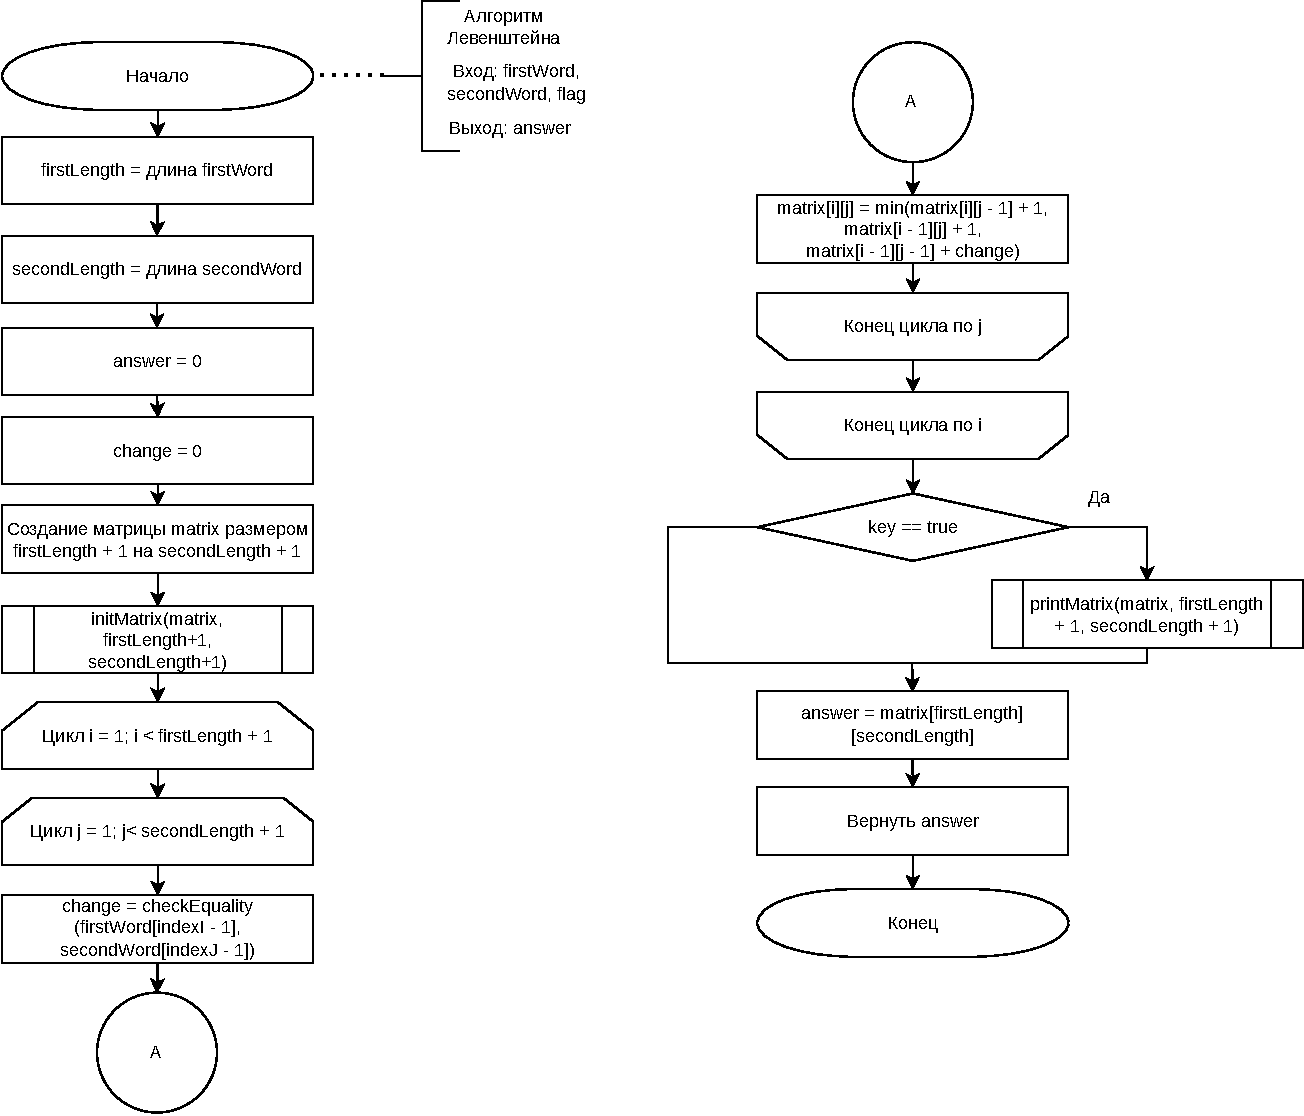
\includegraphics[scale=0.7]{photos/Levenstain.pdf}}
	
	\caption{Схема итеративного алгоритма поиска расстояния Левенштейна}
	
	\label{fig:Levenstain}
\end{figure}

\clearpage

\section{Алгоритмы поиска расстояния Дамерау-Левенштейна}

Рассматриваются итеративный, рекурсивный без кэширования и рекурсивный с кэшированием алгоритмы поиска расстояния Дамерау - Левенштейна.

На рисунках~\ref{fig:DamerauLeven} -- \ref{fig:recursiveCache} приведены схемы рассматриваемых алгоритмов.

\begin{figure}[h]
	
	\centering{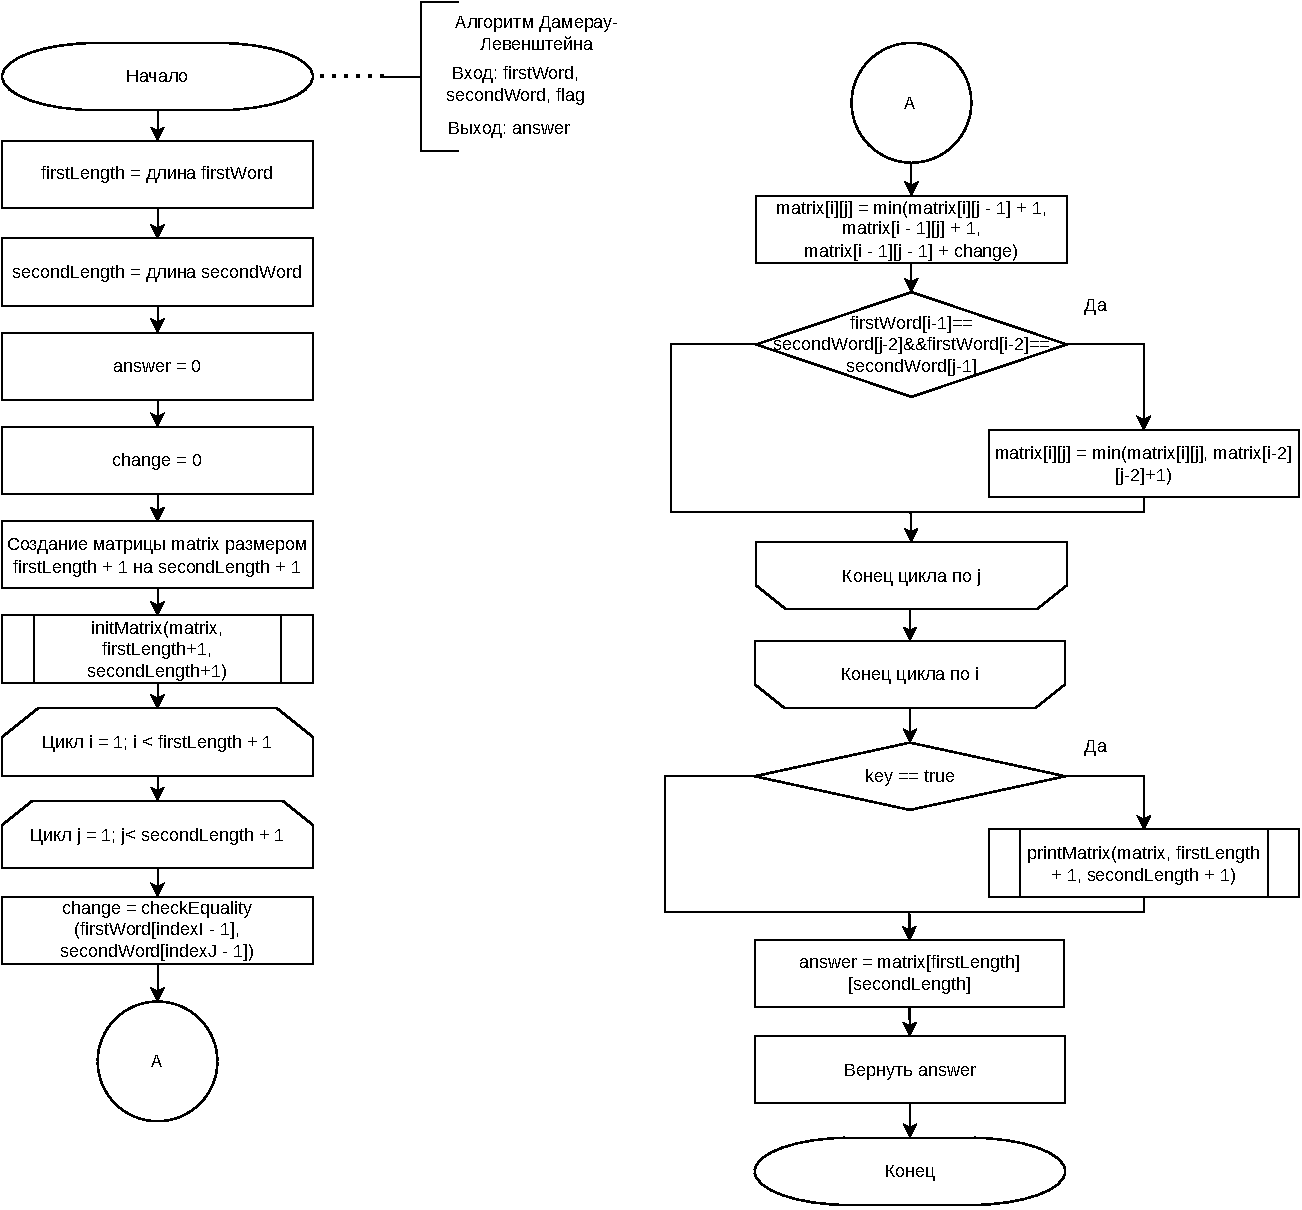
\includegraphics[scale=0.8]{photos/DamerauLeven.pdf}}
	
	\caption{Схема нерекурсивного алгоритма поиска расстояния Дамерау-Левенштейна}
	
	\label{fig:DamerauLeven}
\end{figure}

\clearpage

\begin{figure}[h]
	
	\centering{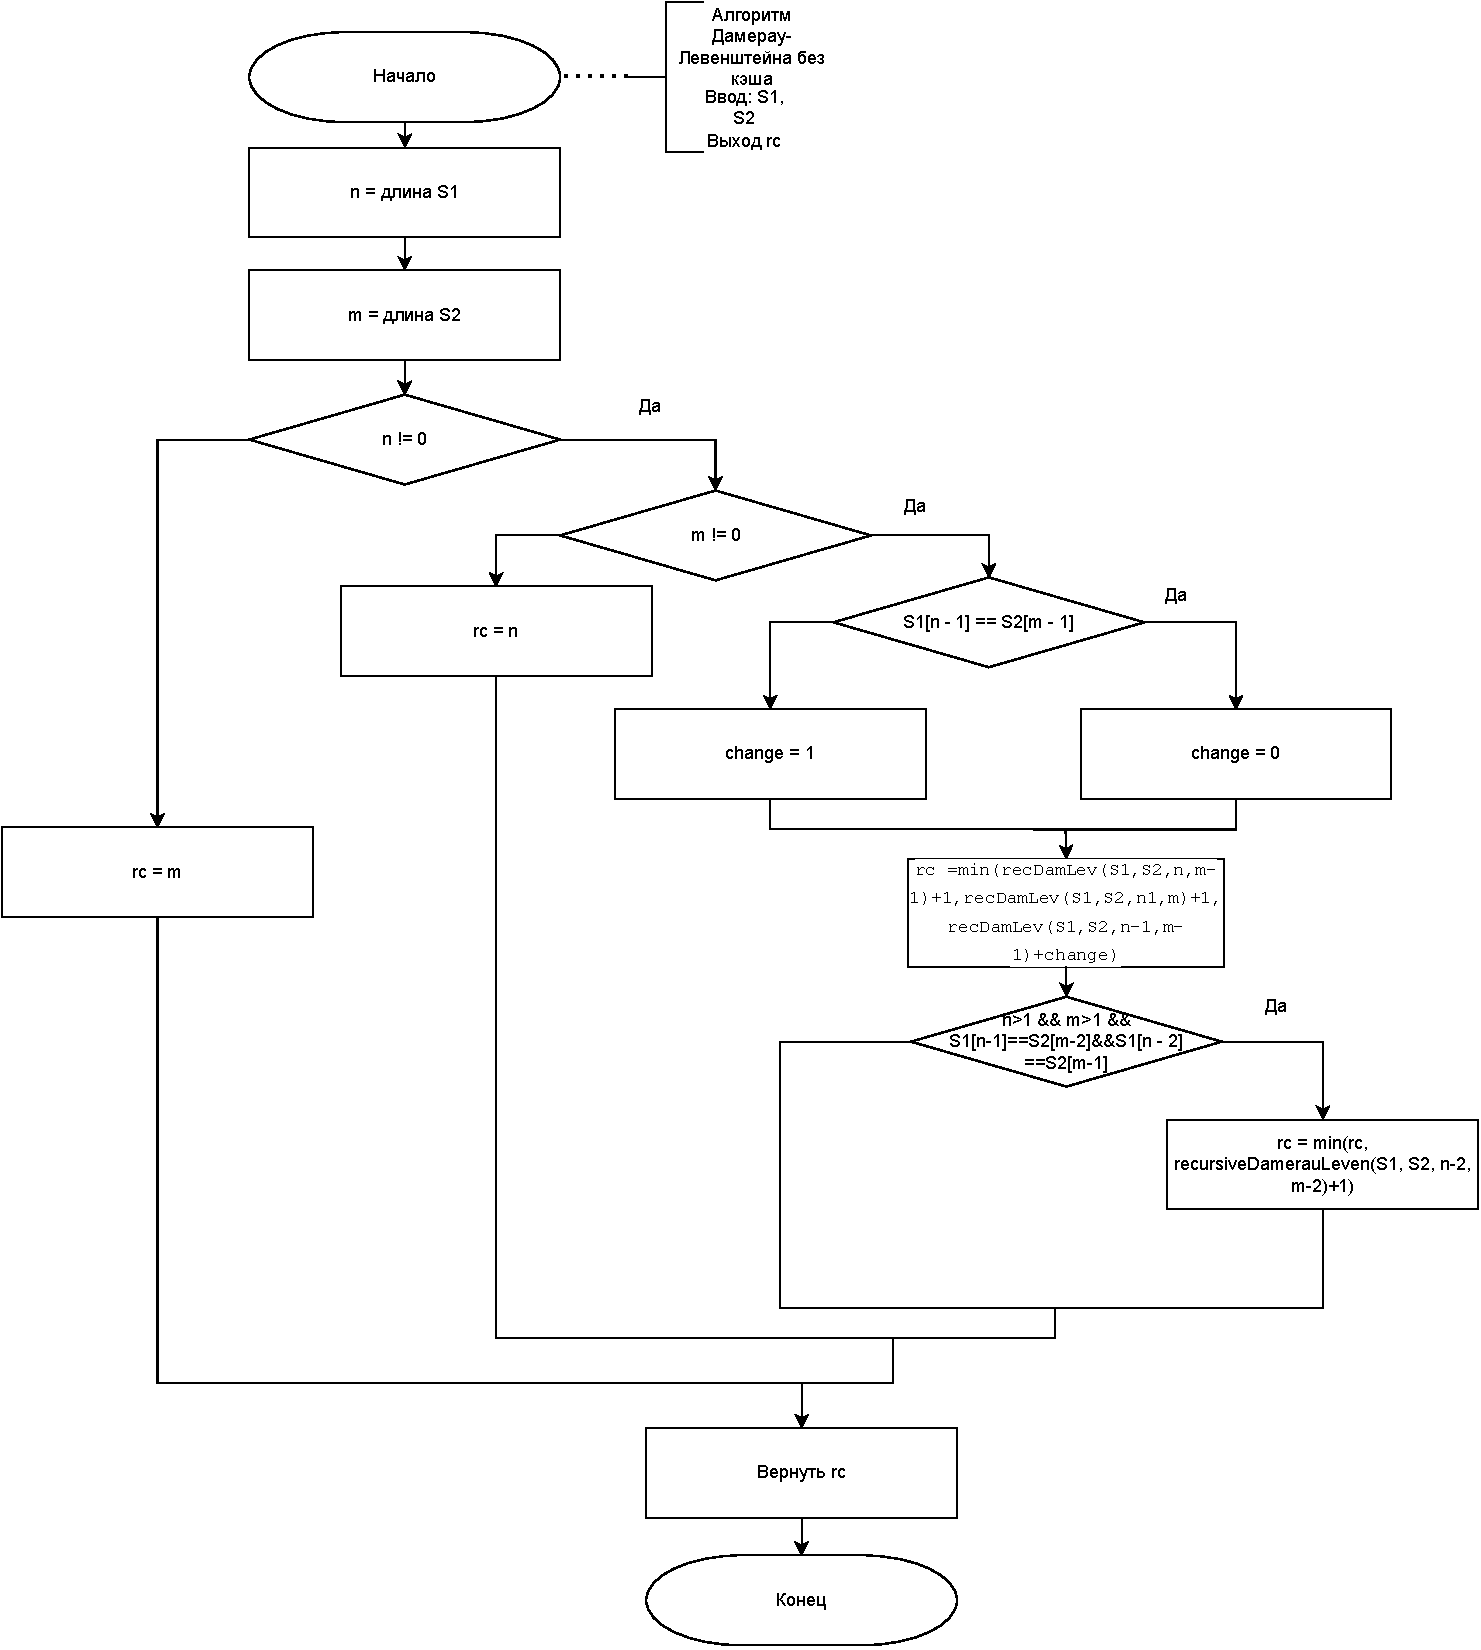
\includegraphics[scale=0.65]{photos/recursive.pdf}}
	
	\caption{Схема рекурсивного алгоритма поиска расстояния Дамерау-Левенштейна без кэширования}
	
	\label{fig:recursive}
	
\end{figure}

\clearpage

\begin{figure}[h]
	
	\centering{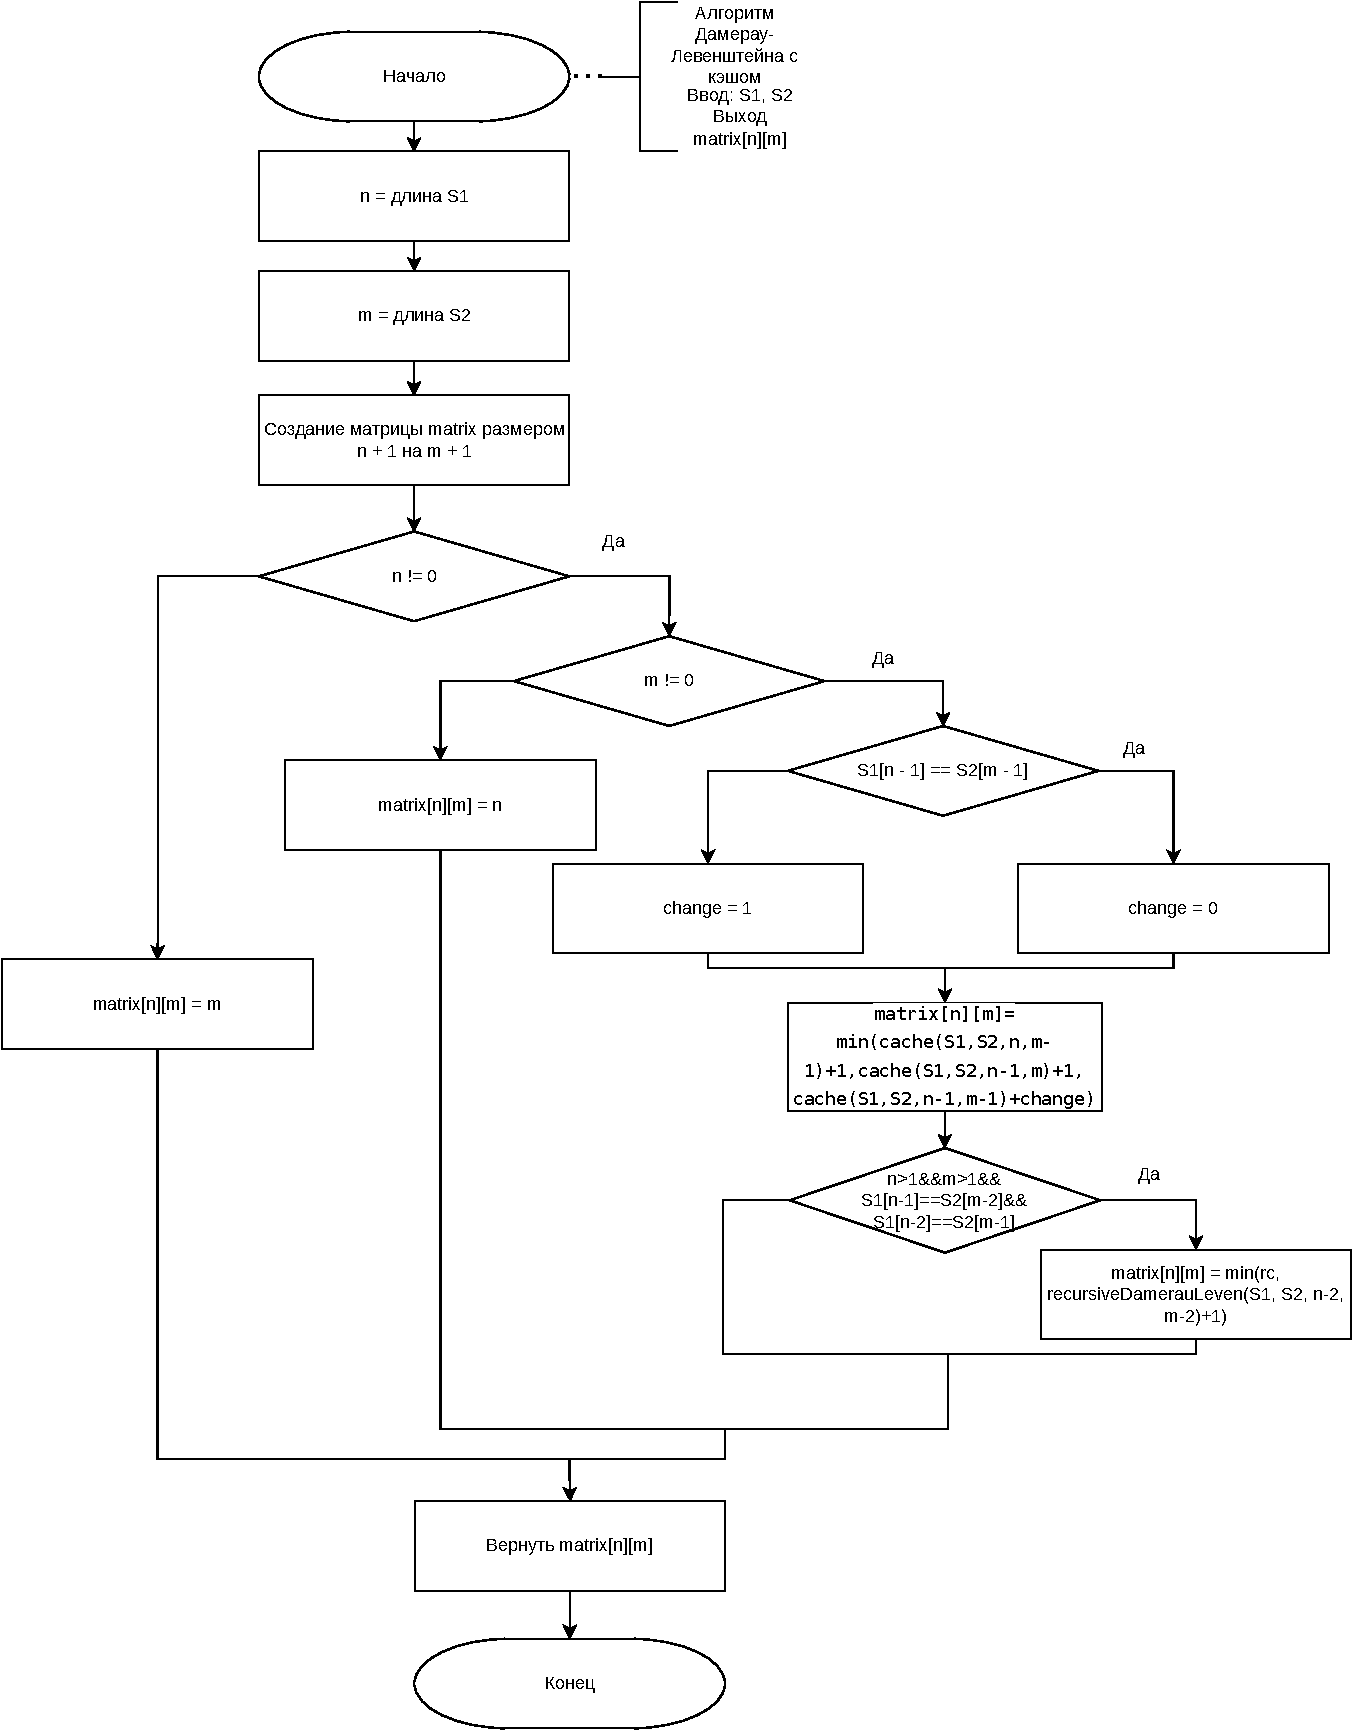
\includegraphics[scale=0.53]{photos/recursiveCache.pdf}}
	
	\caption{Схема рекурсивного алгоритма поиска расстояния Дамерау-Левенштейна с кэшированием}
	
	\label{fig:recursiveCache}
	
\end{figure}

\section*{Вывод}

На основе теоретических знаний, полученных в аналитическом разделе, были разработаны схемы алгоритмов, благодаря которым могут быть найдены расстояния Левенштейна и Дамерау - Левенштейна. 
